\chapter{Theory}
%\subsection{Introduction to Mixing Phenomenology}
\section{Quarks}
In this project, the emphasis lies in explaining of the generation of the masses and mixing of the quarks, the building blocks of matter. Quarks are spin 1/2 fermions that are affected by all three fundamental forces: electromagnetic, strong nuclear, and weak nuclear. They come in 6 different ``flavours'' and they carry fractional charge. Free quarks were never directly observed due to their confinement within hadrons -- composite quark systems. Is is important to note that the definition of mass for the quarks varies according to the renormalisation scheme of the QCD Lagrangian. The only definition of mass that is independent of the adopted renormalisation scheme is quark pole mass (position of the pole in the quark propagator) which is determined by the study of hadron decays and their spectrum using QCD perturbation theory. If desired to be used for phenomenological purposes this can be converted to the running  $\overline{MS}$ renormalisation scheme mass values which can be calculated at three loop order \cite{threepole}. Lattice gauge theory and hence lattice simulations use particular discretization of QCD and lattice spacing to determine a quantity known as bare mass. It is only possible to directly establish the so-called constituent mass which comes from non-relativistic quark models. These can be seen in Table \ref{nonlin}.

\begin{table*} 

\centering % used for centering table 
\begin{tabular}{|c|c|c|c|} % centered columns (4 columns) 
\hline %inserts double horizontal lines 
Generation & ``Flavour" & Charge & Constituent Mass \\ [0.5ex]\hline% inserts table 
%heading 
\hline % inserts single horizontal line 
1st & up  \textit{u}& +2/3 & ~300 Mev/c$^{2}$ \\ % inserting body of the table 
1st & down \textit{d}& -1/3 &  ~300 MeV/c$^{2}$ \\[1ex]
2nd & charm \textit{c}& +2/3 &  ~1.5 Gev/c$^{2}$\\ 
2nd & strange \textit{s}& -1/3 &  ~500 Mev/c$^{2}$ \\[1ex]
3rd & top \textit{t}& +2/3 &  ~175 Gev/c$^{2}$ \\ 
3rd & bottom \textit{b}& -1/3 & ~ 5 Gev/c$^{2}$ \\ [1ex] % [1ex] adds vertical space 
\hline %inserts single line 

\end{tabular} 
\caption{Quarks and their properties} 
\label{nonlin} % is used to refer this table in the text 
\end{table*} 
\section{Lagrangian of the Standard Model}
In order to understand the origin of the mass matrices and their form it is important to introduce some basic aspects of field theories. In quantum field theories, and hence the Standard Model, the dynamics of the system is captured by the most general renormalisable Lagrangian density that is invariant under gauge symmetry. Quantum Chromodynamics (QCD), the field theory that describes the strong interactions of colored quarks and gluons, is the SU(3) component of the Standard Model. Since the strong force is flavour symmetric, this results in mass matrices involving the electroweak interactions only, which are based on the gauge group SU(2)$\otimes$U(1). Both masses and mixing of quarks originate as a result of Yukawa interactions with Higgs condensate \cite{ewconstraint}. Before the spontaneous breakdown of the electroweak symmetry, all quarks and leptons are massless. Once the Higgs scalar field acquires a vacuum expectation value $\langle\phi\rangle = (0, v/\sqrt{2})$ implying broken symmetry, quarks acquire mass and hence the Lagrangian density term involving the mass matrices\cite{texture} is obtained: 
\begin{equation}\label{lama}
{\cal L}_m= -U_{0L}^{\dagger}M_u U_{0R} - D_{0L}^{\dagger}M_dD_{0R} - h.c,
\end{equation}
where $U_{0L}^{\dagger}=(u_0^{*}, c_0^{*}, t_0^{*})_L,\;\; D_{0L}^{\dagger}=(d_0^{*},s_0^{*}, b_0^{*})_L,\;\; U_{0R}^T=(u_0,c_0,t_0)_R,\;\;D_{0R}^T=(d_0,s_0,b_0)_R,$ with $\dagger$ representing conjugate transpose, $T$ transpose and $^{*}$ conjugate. $0$ signifies weak basis eigenstate, $R$ is right-handed quark state, $L$ is left-handed quark state and h.c stands for Hermitian conjugate. $M_{u}$ and $M_{d}$ represent 3 x 3 complex up and down type quark mass matrices containing 36 free parameters. Using polar matrix decomposition, it is possible to decompose  a complex matrix as the product of Hermitian and unitary matrix. Since the unitary matrix can be absorbed into the right-handed quark components, this immediately makes the number of free parameters 18 and $M_{u}$, $M_{d}$  complex Hermitian.
\newline
\indent More suitable, however, is to decompose a complex matrix into two distinguishable unitary and one diagonal matrix. By reverse action mass matrices can be diagonalised by unitary transformations $U_{uL}$ and $ U_{dL}$ in the following way:
\begin{equation}
\begin{split}
\mathcal{M}_{u} = U_{uL}^{\dagger}M_{u}U_{uR} = Diag\{m_{u},m_{c},m_{t}\}
\\
\mathcal{M}_{d} = U_{dL}^{\dagger}M_{d}U_{dR} = Diag\{m_{d},m_{s},m_{b}\}
\end{split}
\end{equation}
\newline
\indent Unitary transformations acting simultaneously on the up and down quark vectors \cite{fritz} to diagonalise mass matrices were used because they are the most general case of a weak basis transformation which transforms a system to different basis without altering the physics, hence giving rise to the same masses and the same CKM matrix and leaving the mass matrices Hermitian. Such transformation is equivalent to changing quark fields from the basis of flavour eigenstates to that of mass eigenstates.
\newline
\indent Due to the diagonalisation of the mass matrices the Lagrangian density term which represents the ( $\text{W}^\pm$ -- mediated) charge current processes involving quarks now includes non diagonal couplings for the current:
\begin{equation}\label{weakcurr}
J_{\mu L}^-= U_{L}^{\dagger}\gamma_\mu V_{CKM}D_{L},
\end{equation}
where  $V_{CKM}= U_u^{\dagger} U_d= U_u^{\dag} U U^{\dag} U_d = U_{uL} U_{dL}^\dag$ is the Cabibbo-Kobayashi-Maskawa (CKM) mixing matrix, which arises as a result of $U_{uR}$ and $U_{dR}$ the unitary matrices diagonalizing the Hermitian $M_uM_u^\dagger$ and $M_dM_d^\dagger$ square mass matrices respectively. $U_{L}^\dagger =( u^{*}, c^{*}, t^{*})_L$ and $D_{L}^T=(d,s,b)_L$ are now the quark field mass eigenstates. So the complete electroweak Lagrangian includes both equations \ref{lama} and \ref{weakcurr}.

\section{Quark Mixing Matrix}
\indent As mentioned above, from transformation of mass matrices via two unitary matrices one obtains the Cabibbo-Kobayashi-Maskawa matrix. Experimentally there is a strong hierarchy in the size of the matrix elements of the quark mixing matrix. The origin of this hierarchy, however, is still an unsolved puzzle. In the literature, there  are several approaches to solving this problem, one of them being to search for simple textures of quark matrices that can predict self-consistent and experimentally favoured relations between quark masses and flavour mixing parameters. 
\newline 
\indent The quark mixing matrix is a $3 \times 3$ complex unitary matrix. Hence, there are 18 parameters to start with. Unitarity of the CKM matrix implies that matrix elements are orthonormal, reducing the count of free parameters to 9. Further, 5 out of 6 quark phases can be absorbed into the redefinition of the quark field, cutting the number of parameters down to 4 parameters, three quark mixing angles and one CP violating phase\cite{book}.
\newline
\indent There are many different parametrisations\cite{param} which are all mathematically equivalent to the CKM matrix, but the standard parametrisation of the CKM matrix for flavour mixing is the following:


\begin{align}
V_{\rm CKM} &=  \begin{pmatrix}   V_{ud} & V_{us} & V_{ub} \cr
    V_{cd} & V_{cs} & V_{cb} \cr
    V_{td} & V_{ts} & V_{tb} \cr \end{pmatrix} \\
 &= \begin{pmatrix}c_{12}c_{13}& s_{12}c_{13} & s_{13}\exp(-i\delta) \cr
-s_{12}c_{23}-c_{12}s_{23}s_{13}\exp(i\delta) & c_{12}c_{23}- 
s_{12}s_{23}s_{13}\exp(i\delta) & s_{23}c_{13} \cr 
s_{12}s_{23}- c_{12}c_{23}s_{13}\exp(i\delta) & 
-c_{12}s_{23}-s_{12}c_{23}s_{13}\exp(i\delta) & c_{23}c_{13}\end{pmatrix},
\end{align}

where $s_{ij} = \sin(\theta_{ij})$ and $c_{ij} = \cos(\theta_{ij})$, $\theta_{12}$ , $\theta_{23}$, $\theta_{13}$ are Euler angles and $\theta_{12}$ is also known as the Cabibbo angle.
A parametrisation reflecting the hierarchical nature in flavour mixing, which is an expansion in terms of the small parameter $\lambda$, was introduced by Wolfenstein\cite{wolf}. The four Wolfenstein parameters, which will be of paramount interest in exploring one of the ans\"{a}tze for the mass matrices, are related to the standard parametrization via the following expressions:
\begin{equation}
\begin{split}
\lambda = s_{12}, \\
\qquad
A\lambda^{2} = s_{23}, \\
\qquad
A\lambda^{3}(\rho - i\eta) = s_{13}exp(-i\delta),\\
\end{split}
\end{equation}

\begin{equation}V_{\rm CKM_{Wolfenstein}} = \begin{pmatrix}1-\lambda^2/2 & \lambda & A\lambda^3(\rho-i\eta) \cr
 -\lambda & 1-\lambda^2/2 & A\lambda^2 \\
 A\lambda^3(1-\rho-i\eta) & -A\lambda^2 & 1\end{pmatrix} + {\cal O}\left( \lambda^4 \right). \
\end{equation}


\indent A geometrical interpretation of $CP$ violation is offered by the concept of unitarity triangles. Unitarity of the CKM matrix can be summarized by two sets of orthogonality relations:
$\sum_{k} |V_{ik}|^2 = \sum_{i} |V_{ik}|^2 = 1$ for all $i$ generations and $\sum_k V_{ik}V^*_{jk} = 0$ for all $i\neq j$. One of the unitary constraints of the CKM matrix explicitly states:
\begin{equation}
  V_{ud}V^*_{ub} + V_{cd}V^*_{cb} + V_{td}V^*_{tb} = 0 \, .
\end{equation}
If you divide this expression by 
\begin{equation}
V_{cd}V^*_{cb}
\end{equation}
and take relation\cite{Buras} of $\bar{\rho}$ and $\bar{\eta}$ to ${\rho}$ and ${\eta}$ 
\begin{equation}
   {\rho} + i {\eta} = \frac{\sqrt{A^{4}\lambda^{4}}(\bar{\rho} + i \bar{\eta})}{\sqrt{1-\lambda^2}[A^{4}\lambda^{4}(\bar{\rho} + i \bar{\eta})]}
\end{equation}
and definition of $\bar{\rho}$ and $\bar{\eta}$
\begin{equation}
\bar{\rho} \approx \rho - \frac{\rho\lambda^{2}}{2}
\end{equation}
\begin{equation}
\bar{\eta} \approx \eta - \frac{\eta\lambda^{2}}{2}
\end{equation}

  it can be pictorially represented \cite{ewconstraint} in the $\bar{\rho}$ and $\bar{\eta}$ plane as in Figure 1.
%\begin{figure*}[t]
%\caption{Unitarity triangle in a complex plane.}
%  \centering
%    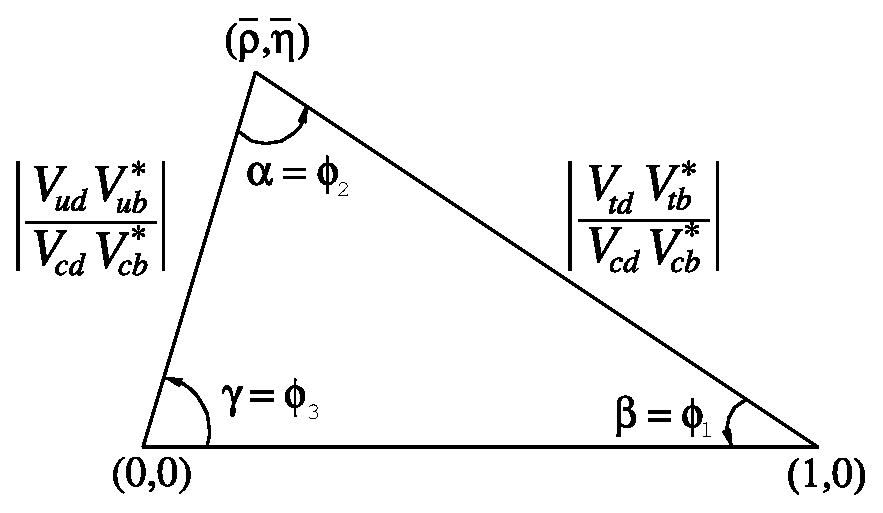
\includegraphics[width=0.5\textwidth]{triangle2.eps}
%\end{figure*}

The area of these triangles are half of the Jarlskog invariant \textit{J}, a quantifier of CP violation, which is defined as $ Im[V_{ij}V_{kl}V^*_{il}V^*_{kj}]$ \cite{jarsklog}. It is independent of phase convention. It is important to emphasize that the Standard Model with its parameters may or may not violate CP. Only after measuring the parameter it is possible to determine the CP non-conservation. \textit{J} vanishes\cite{secondjar} only if mixing angle $\theta_{ij} = 0 , \pi/2$; $\delta =  0 , \pi$; So measurements of \textit{J} allows to verify that the CKM matrix is complex and hence different mixing for quarks and anti-quarks is obtained, providing theoretical grounding for CP violation, one of the Sakharov conditions for the evolution of the universe which we see today, although the standard model CP violation is not big enough to explain the matter dominated universe.

Experimentally the most precise measurement of the CKM matrix\cite{ewconstraint} to-date is 
%\begin{equation}|V_{\rm CKM}| = \begin{pmatrix}0.97427 \pm 0.00015 & 0.22534 \pm 0.00065  &  0.00351\pm \bfrac{0.00015}{0.00014} \cr
%0.22520 \pm 0.00065 &  0.97344 \pm 0.00016 & 0.0412\pm\bfrac{0.0011}{0.0005} \cr
%0.00867 \pm \bfrac{0.00029}{0.00031} & 0.0404 \pm \bfrac{0.0011}{0.0005} &  0.999146 \pm \bfrac{0.000021}{0.000046} \cr \end{pmatrix} .
%\end{equation}

\section{Fully Leptonic $P^{+}\rightarrow l^{+} \nu_{l}$ decays}
This text is based on a summary provided by PDG on Leptonic Decays of Charged Pseudoscalar Mesons.


Purely leptonic decays that proceed by annihilation-type diagrams of pseudoscalar mesons ($P$) are of great interest for flavour physicists because of several reasons as they allow:
\begin{itemize}
\item measurements of the CKM matrix elements,
\item measurements of leptonic decay constants,
\item measurements of the new physics effects.
\end{itemize}



First two types of measurements are possible because the decay rates of $P^{+}\rightarrow l^{+} \nu_{l}$ decays are sensitive to the product of the appropriate CKM matrix element ($V_{q_{1}q_{2}}$ where $q_{1}$ and $q_{2}$ are constituent quarks of the pseudoscalar meson) and decay constant $f_{P}$, related parameter arising from the strong interaction. In more detail, the decay width of fully leptonic decay of a pseudoscalar meson in the Stadard Model to the lowest order can expressed as 

\begin{equation}
%\label{eqn:br} 
\Gamma(P^{+} \rightarrow {l^{+}} \nu_{l})=  
	\frac{G_{F}^{2} m^{}_{P^{+}}  m_{l^{+}}^{2}}{8\pi} 
	\left[1 - \frac{m_{l^{+}}^{2}}{m_{P^{+}}^{2}}\right]^{2}  
	f_{P}^{2} |V_{q_{1}q_{2}}|^{2} 
	,
\label{eqn:dw} 
\end{equation}

where
$G_F$ is the Fermi constant,
$m^{}_{P^{+}}$ and $m_{l^{+}}$ are the pseudoscalar meson and lepton masses, respectively,
$\tau_{P^{+}}$ is the $P^{+}$ lifetime.

So in order to measure CKM matrix amplitude, knowledge of $f_{P}$ must be inferred. $f_{P}$ can be calculated using lattice QCD techniques and together with experimental determination of the decay rates provides provide a way to determine relevant amplitude squared of the relevant CKM matrix element. More conventionally, CKM magnitudes are determined from semileptonic decays, but in this case the sensitivity to different type of current is given. In purely leptonic decays axial-vector flavour-changing currents ($q_{1}\gamma_{\mu}\gamma_{5}q_{2}$) are probed as opposed to vector current ($q_{1}\gamma_{\mu}q_{2}$) in semileptonic case.

Vice versa, assuming unitarity of CKM triangle and experimental determination of relevant $V_{q_{1}q_{2}}$ one can obtain experimental determination of the decay constants and compare it with theoretical prediction.

Last, but not least, is of course the measurement of presence of new physics in these decays. Especially appealing is the presence of new particles which would manifest themselves in the decay rates of heavier pseudoscalars ($D_{(s)}$ or $B$). Example of such new particles include charged Higgs bosons, $H^{\pm}$, coming from so-called Type II of two-Higgs-doublet models \cite{Hou:1992sy}\cite{Akeroyd:2003zr}\cite{Dobrescu:2008er} or leptoquarks\cite{Dobrescu:2008er}. In this case, considering $B^{+}\rightarrow l^{+}\nu$ decay, four-fermion interaction between $W^{\pm}$ and $H^{\pm}$ would modify the SM decay width~\autoref{eqn:dw} to
%remember branching fraction is partial width of total width
%total width  h over liftime so lifetime is always missing from equations 
% see https://www2.ph.ed.ac.uk/~vjm/Lectures/ParticlePhysics2010_files/Particle3-2Nov.pdf this

\begin{equation}
\Gamma(B^{+} \rightarrow {l^{+}} \nu_{l})=  
        \frac{G_{F}^{2} m^{}_{B^{+}}  m_{l^{+}}^{2}}{8\pi} 
        \left[1 - \frac{m_{l^{+}}^{2}}{m_{B^{+}}^{2}}\right]^{2}  
	f_{P}^{2} |V_{ub}|^{2} \,\times\, r_H,
%\Gamma(B^+\to \ell^+\nu_\ell)={G_F^2 m_{B} m_l^2 f_{B}^2\over 8\pi}
%|V_{ub}|^2 \left(1-{m_l^2\over m^2_{B}}\right)^2 \,\times\, r_H
\end{equation}

where
\begin{equation}
	r_H=[1-\tan^2\beta(m^{2}_{B^{+}}/m^{2}_{H^{+}})]^2.
\end{equation}

Here $\tan\beta = \frac{v_{2}}{v_{1}}$, where $v_{i}$ are the vacuum expectation values for the Higgs doublets. In order to have enhancing effect for the rate of $B^{+}\rightarrow l^{+}\nu$ decay (to have $r_{H}>1$), $\tan\beta/H^{\pm}> 0.27 \gev^{-1}$.

Given current tensions arising in flavour physics searches especially concerning lepton non-unversality, ratio of rates between $P\rightarrow\tau\nu$,$P\rightarrow\mu\nu$ and $P\rightarrow e\nu$ should be measured. In the ratios the decay constant $f_{P}$ cancels out making such measurements good tool for lepton universality tests.

As seen in~\autoref{eqn:dw}, purely leptonic final state going through $P\rightarrow W^{*}\rightarrow l \nu$ is supressed by $m^{2}_{l}$, also known as helicity supression. This suppression occurs as a result of angular momentum conservation. In case of $B^{+}\rightarrow l^{+} \nu$, $B^{+}$ is a spin-0 particle and hence its decay products have to have spin 0 combined, or in other words, be anti-aligned. Neutrinos in the SM are always produced left-handed. As the spin of the antilepton and the neutrino should be anti-aligned, antilepton also needs to be left-handed (to have negative helicity). However, the weak current only couples to right-handed antiparticles. Therefore, the antilepton has to be boosted in order to have different helicity. For massless particles such helicity flip is not possible making this decay impossible. The lighter the lepton the larger the velocity and hence higher boost is necessary, making decays to lighter leptons rarer even though they have bigger kinematic phase space available.

%https://www.physicsforums.com/threads/helicity-and-suppression.804600/
The latest experimental measurements for rates of these measurements have been performed by $B$ factories, finding evidence for $B^{+}\rightarrow \tau^{+}\nu$ and first sign of $B^{+}\rightarrow \mu^{+}\nu$ as seen in~\autoref{tab:sum}. These results are to be compared with SM prediction $\mathcal{B}(B^{+}\rightarrow \tau^{+}\nu) = (0.82+0.03-0.02)\times10^{-4}$\cite{Charles:2004jd} which is obtained by using unitarity-constrained $V_{ub}$ value aggregated from other measurements and lattice calculations of $f_{B}$. Quite subtantial statistical as well as systematical errors show the difficulty of this type of measurements. 

\begin{table}[ht]
\begin{center}
\begin{tabular}{ l l l l H c H} \hline
	Process &Experiment & Tag &${\mathcal{B}}$ ($\times$ $10^{-4}$) & Published & Significance ($\sigma$) & {$|V_{ub}|f_{B^+}$ (MeV)} \hfill\\
\hline\\[-2.5ex]
	$B^{+}\rightarrow \tau^{+}\nu$	&Belle~\cite{Adachi:2012mm}&Hadronic&$0.72^{+0.27}_{-0.25}\pm0.11$  & 2013 & 3.0 \\ 
$B^{+}\rightarrow \tau^{+}\nu$	&Belle~\cite{Kronenbitter:2015kls}&Semileptonic&$1.25\pm0.28\pm0.27$ & 2015 & 3.8 \\
$B^{+}\rightarrow \tau^{+}\nu$	&Belle~\cite{Kronenbitter:2015kls}&Average&$0.91 \pm 0.22$ & 2015 & 4.6 \\\hline\\[-2.5ex]
$B^{+}\rightarrow \tau^{+}\nu$	&BaBar~\cite{Lees:2012ju} & Hadronic & $1.83\,^{+0.53}_{-0.49}\pm0.24$ & 2012 & 3.8 \\ 
$B^{+}\rightarrow \tau^{+}\nu$	&BaBar~\cite{Aubert:2009wt} & Semileptonic & $1.7\pm 0.8\pm 0.2$ & 2010 & 2.3\\ 
$B^{+}\rightarrow \tau^{+}\nu$	&BaBar~\cite{Lees:2012ju} & Average & $1.79 \pm 0.48$ & 2012 & - & $1.01\pm 0.14$  \\ \hline
$B^{+}\rightarrow \mu^{+}\nu$ & Belle~\cite{Sibidanov:2017vph} & Untagged& $(6.46\pm2.22\pm 1.60)\times 10^{-3}$ & 2017 & 2.4 &\\
%        & Our average & &$1.06\pm0.20$&$0.77\pm0.07$ & & \\
\hline
\end{tabular}
\end{center}
\caption{Experimental summary of searches for $B^{+}\rightarrow l^{+}\nu$.}
\label{tab:sum}
\end{table}


With helicity supressed rates and very limited signature in the detector (one chaged track for muons and electron, more charged tracks for taus, but also more missing energy depending on the reconstruction channel) searching for such decays is still very challenging. In order to make measurements of the same kind (CKM precision measurements, decay constants measurements, new physics searches), fully leptonic decays but with photons can be considered.   

\section{Fully Leptonic $B^{+}\rightarrow l^{+} \nu_{l} \gamma$ decays}
The helicity suppression can be lifted by considering the decay with an additional photon radiated from the $B^{+}$ meson, at the cost of the electromagnetic suppression with coupling constant $\alpha_{em}$. Consequently, the branching fraction for radiative decays can be comparable or even larger than the corresponding fraction for purely leptonic decays. It has been shown that $R^{\mu}_{B}=\frac{\Gamma(B\rightarrow \mu \nu \gamma)}{\Gamma(B\rightarrow \mu \nu)}\approx(1-20)$ making $\mathcal{B}(B\rightarrow \mu \nu \gamma)\approx(10^{-7}-10^{-6})$ \cite{Burdman:1994ip}.

The differential decay width with $\frac{1}{m_{b}}$ and radiative corrections
at next-to-leading logarithmic order calculated in\cite{Beneke:2011nf} is given by the following formula:
\begin{equation}
\frac{d\Gamma}{dE_{\gamma}} = \frac{\alpha_{em}G^{2}_{F}|V_{ub}|^{2}}{48 \pi^{2}}m_{B}^{4}(1 - x_{\gamma})x_{\gamma}^{3}[F_A^{2} + F_V^{2}]
\end{equation}
 where $x_{\gamma} = 2E_{\gamma}/m_{B}$, $F_A$ is axial form factor and $F_V$  is vector form factor defined as
\begin{equation}
F_{V}(E_{\gamma}) = \frac{Q_{u}m_{B}f_{B}}{2E_{\gamma}\lambda_{B}(\mu)} R(E_{\gamma}, \mu) + [\xi(E_\gamma) +  \frac{Q_{u}m_{B}f_{B}}{(2E_{\gamma})^{2}} + \frac{Q_{b}m_{B}f_{B}}{2E_{\gamma}m_{b}}],
\end{equation}

\begin{equation}
F_{A}(E_{\gamma}) = \frac{Q_{u}m_{B}f_{B}}{2E_{\gamma}\lambda_{B}(\mu)} R(E_{\gamma}, \mu) + [\xi(E_\gamma) -  \frac{Q_{u}m_{B}f_{B}}{(2E_{\gamma})^{2}} - \frac{Q_{b}m_{B}f_{B}}{2E_{\gamma}m_{b}} + \frac{Q_{l}f_{B}}{E_{\gamma}}].
\end{equation}
Here $Q_{l},Q_{u},Q_{b}$ are the charges of the lepton, up quark, and
bottom quark, respectively, $f_{B}$ is the decay constant for
the B meson, and $R(E_{\gamma}, \mu)$ is a radiative correction
calculated at the energy scale $\mu$ %that equals one at tree level.
and $m_{b}$ is the mass of $b$ quark.

The term not in squared brackets represents the leading-power contribution in the heavy-quark expansion. Note that this term
is the same for the vector and axial form factor. The terms in square brackets are $\frac{1}{m_{b}}$ power corrections relative to the leading term. Further corrections have been discussed in~\cite{Wang:2016beq}.



Recent measurement of the radiative $B^{+} \rightarrow l^{+} \nu_{l} \gamma$, where $l^{+}$ is either $e^{+}$ or $\mu^{+}$ was performed by Belle using hadronic tagging on their full data sample\cite{Heller:2015vvm}.The search yielded $\mathcal{B}(B^{+}\rightarrow \mu^{+} \nu_\mu \gamma) < 3.4\times 10^{-6}$ \cite{Heller:2015vvm}.



\section{Fully Leptonic $B^{+}\rightarrow l^{+} l^{-} l^{+} \nu_{l} $ decays}

In LHCb, the most optimal approach due to the detector capabilities is to measure this kind of decay by decaying the photon into pair of muons, see~\autoref{fig:myfeyn}(a). This though introduces suppression by $\alpha_{em}$. If the naive expectation of only taking into account photon conversion into two muons is adopted, then the expected branching fraction for this analysis is $\mathcal{B}(B^{+}\rightarrow \mu^{+} \mu^{-} \mu^{+} \nu_{\mu}) \approx 10^{-8}$ (will be referred to as pessimistic BF). However this estimate is of course not correct because there are other contributions to the total branching fraction as it was shown in the first theoretical prediction for $\mathcal{B}(B^{+}\rightarrow \mu^{+} \mu^{-} \mu^{+} \nu_{\mu})$.

The first theoretical prediction published for the $\mathcal{B}(B^{+} \rightarrow \mu^{+} \mu^{-} \mu^{+} \nu_{\mu})$ decay branching fraction\cite{Danilina:2017bcn} yields approximately $1\times 10^{-7}$ where the majority of the contribution actually comes from the $\rho$ and $\omega$ resonances, which are included as a part of the signal (will be referred to as optimistic BF). An example of of such contribution can be seen in~\autoref{fig:myfeyn}(b), where \Bmumumu proceeds via the hadronic contributions to the photon pole.

%\begin{figure}[here]
%\includegraphics[scale=0.5]{theory/newfeyn4}\put(-30,133){(a)}
%\includegraphics[scale=0.5]{theory/btorhomunurad}\put(-30,133){(b)}
%\centering
%\caption{(a) Annihilation diagram where the initial state quark radiates off a virtual photon which decays into a pair of muons with small invariant mass ($q^{2}$) and the $W^{+}$ turns into a muon and muon neutrino. (b) Most of the contribution to the rate comes from hadronic contribution to photon.}
%\label{fig:myfeyn}
%\end{figure}






